\begin{lstlisting}[language=c++]
//FLOPs FOR ACCELERATION
// 1 FLOP * 3 directions
dx = x1 - x2
// 3 FLOPs
r = sqrt(dx*dx + dy*dy + dz*dz)
// 7 FLOPs
a = - (Gconst*m*M/(r*r)) / (m*r)
// 2 FLOPs * 3 directions
a = a + a*(x1-x2);																	
//TOTAL FLOPs = 19 FLOPs 


//FLOPs FOR POSITION :: EULER
// 2 FLOPs * 3 directions
x = x + t_step*Vx															
//TOTAL FLOPs = 6 FLOPs 


//FLOPs FOR VELOCITY :: EULER
// 2 FLOPs * 3 directions
Vx = Vx + t_step*ax															
//TOTAL FLOPs = 6 FLOPs 


//FLOPs FOR POSITION :: Verlet
// 6 FLOPs * 3 directions
x = x + t_step*Vx + (0.5*t_step*t_step*a);
//TOTAL FLOPs = 21 FLOPs


//FLOPs FOR VELOCITY :: Verlet
// 4 FLOPs * 3 directions
Vx = Vx + (0.5*t_step*(Ax+Ax_old));
//TOTAL FLOPs = 12 FLOPs
\end{lstlisting}

\pagebreak

\begin{figure}[H]
		\centering
		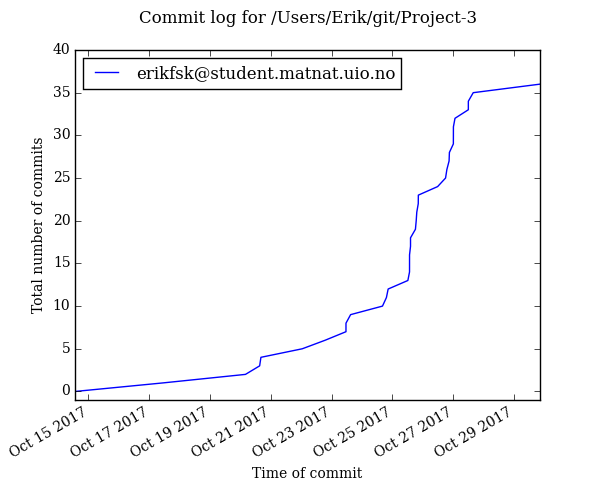
\includegraphics[width=0.7\linewidth]{appendix/bilder/workflow.png}
		\caption{Our retarded workflow... Next time maybe it will be better?}
		\label{fig:ab}
\end{figure}